\section{Méthodologie}

\subsection{Framework DFA-IA}

\subsubsection{Concept Général}

Le framework DFA-IA (Design For AI - Intelligence Artificielle) proposé par DesignPro AI s'inspire du processus traditionnel de développement de produit tout en y intégrant l'intelligence artificielle générative à des points stratégiques. La figure \ref{fig:framework} illustre ce framework.

\begin{figure}[H]
\centering
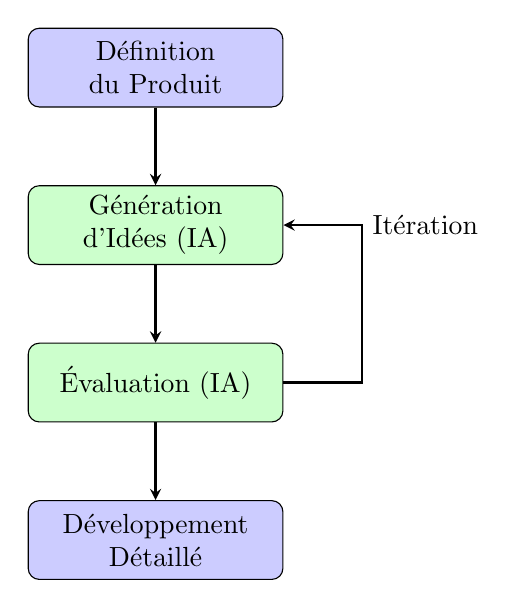
\begin{tikzpicture}[
    node distance=2cm,
    box/.style={rectangle, draw, fill=blue!20, text width=3cm, text centered, rounded corners, minimum height=1cm},
    ai/.style={rectangle, draw, fill=green!20, text width=3cm, text centered, rounded corners, minimum height=1cm},
    arrow/.style={->, >=stealth, thick}
]
    \node[box] (def) {Définition du Produit};
    \node[ai, below of=def] (gen) {Génération d'Idées (IA)};
    \node[ai, below of=gen] (eval) {Évaluation (IA)};
    \node[box, below of=eval] (dev) {Développement Détaillé};
    
    \draw[arrow] (def) -- (gen);
    \draw[arrow] (gen) -- (eval);
    \draw[arrow] (eval) -- (dev);
    \draw[arrow] (eval.east) -- ++(1,0) |- (gen.east) node[midway, right] {Itération};
\end{tikzpicture}
\caption{Framework DFA-IA intégrant l'IA générative}
\label{fig:framework}
\end{figure}

\subsubsection{Intégration de l'IA dans le Processus de Design}

DesignPro AI intègre l'IA générative dans les trois premières étapes du processus de conception :

\begin{enumerate}[leftmargin=*]
    \item \textbf{Définition du Produit} : L'utilisateur spécifie les besoins, le domaine d'application, et les contraintes
    
    \item \textbf{Génération d'Idées} : L'IA génère des concepts visuels basés sur :
    \begin{itemize}
        \item Des prompts optimisés (Mistral AI)
        \item Des méthodologies de design (TRIZ, Design Thinking, DFX, Value Engineering)
        \item Des modèles de diffusion (Stable Diffusion XL, ControlNet)
    \end{itemize}
    
    \item \textbf{Évaluation} : L'IA évalue les concepts générés selon :
    \begin{itemize}
        \item Des critères esthétiques et fonctionnels (Agent Q)
        \item Des contraintes de fabrication (R.E.A.L.)
        \item Des principes DfX sélectionnés
    \end{itemize}
\end{enumerate}

\subsection{Pipeline Complet}

Le pipeline de DesignPro AI se décompose en 6 étapes séquentielles, illustrées dans la figure \ref{fig:pipeline}.

\begin{figure}[H]
\centering
\begin{tikzpicture}[
    node distance=1.5cm,
    step/.style={rectangle, draw, fill=blue!15, text width=2.5cm, text centered, minimum height=0.8cm, font=\small},
    arrow/.style={->, >=stealth, thick}
]
    \node[step] (p1) {1. Génération Prompt};
    \node[step, right of=p1, xshift=2cm] (p2) {2. Chargement Modèle};
    \node[step, right of=p2, xshift=2cm] (p3) {3. ControlNet (opt.)};
    \node[step, below of=p3, yshift=-0.5cm] (p4) {4. Génération Image};
    \node[step, left of=p4, xshift=-2cm] (p5) {5. Post-traitement};
    \node[step, left of=p5, xshift=-2cm] (p6) {6. Rapport DfX};
    
    \draw[arrow] (p1) -- (p2);
    \draw[arrow] (p2) -- (p3);
    \draw[arrow] (p3) -- (p4);
    \draw[arrow] (p4) -- (p5);
    \draw[arrow] (p5) -- (p6);
\end{tikzpicture}
\caption{Pipeline de génération et évaluation}
\label{fig:pipeline}
\end{figure}

\subsubsection{Étape 1 : Génération de Prompt}

L'utilisateur fournit des informations de haut niveau :
\begin{itemize}[leftmargin=*]
    \item Catégorie de produit (meuble, électronique, automobile, etc.)
    \item Focus du design (ergonomie, esthétique, fonctionnalité, etc.)
    \item Style visuel (minimaliste, industriel, futuriste, etc.)
    \item Méthodologie de design (TRIZ, Design Thinking, DFX, Value Engineering)
\end{itemize}

Mistral AI génère alors un prompt détaillé et optimisé pour Stable Diffusion, intégrant :
\begin{itemize}[leftmargin=*]
    \item Des descriptions visuelles précises (formes, matériaux, textures)
    \item Des contraintes de la méthodologie choisie
    \item Des paramètres de rendu (éclairage, angle de vue, style photographique)
\end{itemize}

\subsubsection{Étape 2 : Chargement du Modèle}

Le système sélectionne et charge le modèle de diffusion approprié :

\begin{table}[H]
\centering
\caption{Modèles de génération d'images disponibles}
\label{tab:models}
\begin{tabular}{@{}lll@{}}
\toprule
\textbf{Modèle} & \textbf{Résolution} & \textbf{Cas d'usage} \\ 
\midrule
Stable Diffusion 1.5 & 512×512 & Génération rapide, équilibre qualité/vitesse \\
Stable Diffusion 2.1 & 512×512 & Meilleure cohérence des détails \\
Stable Diffusion XL & 1024×1024 & Haute qualité, photoréalisme \\
SDXL Turbo & 1024×1024 & Génération ultra-rapide (itération) \\
OpenJourney v4 & 512×512 & Style artistique (Midjourney-like) \\
\bottomrule
\end{tabular}
\end{table}

\subsubsection{Étape 3 : ControlNet (Optionnel)}

Pour le mode sketch-to-image, ControlNet \cite{zhang2017controlnet} est utilisé pour guider la génération :

\begin{itemize}[leftmargin=*]
    \item \textbf{Prétraitement} : Détection de contours Canny sur le sketch
    \item \textbf{Guidage} : ControlNet contraint la génération à respecter la structure du sketch
    \item \textbf{Flexibilité} : Le paramètre \texttt{controlnet\_conditioning\_scale} (0-1) contrôle la fidélité au sketch
\end{itemize}

\subsubsection{Étape 4 : Génération d'Image}

Le modèle de diffusion génère l'image via un processus de débruitage itératif :

\begin{algorithm}[H]
\caption{Processus de génération par diffusion}
\begin{algorithmic}[1]
\State $x_T \sim \mathcal{N}(0, I)$ \Comment{Bruit gaussien initial}
\For{$t = T$ \textbf{to} $1$}
    \State $\epsilon_\theta \gets \text{UNet}(x_t, t, c)$ \Comment{Prédiction du bruit}
    \State $x_{t-1} \gets \text{Denoise}(x_t, \epsilon_\theta, t)$ \Comment{Débruitage}
\EndFor
\State \Return $x_0$ \Comment{Image finale}
\end{algorithmic}
\end{algorithm}

Où $c$ représente le conditioning (prompt encodé + ControlNet si applicable).

\subsubsection{Étape 5 : Post-traitement}

L'image générée subit un post-traitement minimal :
\begin{itemize}[leftmargin=*]
    \item Conversion du format (tensor → PIL Image)
    \item Encodage en Base64 pour l'affichage web
    \item Sauvegarde dans Supabase Storage
\end{itemize}

\subsubsection{Étape 6 : Génération de Rapport DfX}

Mistral AI génère un rapport DfX basé sur :
\begin{itemize}[leftmargin=*]
    \item L'aspect DfX sélectionné (DFA, DFM, DFS, DFSust)
    \item L'analyse visuelle de l'image (GPT-4 Vision)
    \item Le prompt et la méthodologie utilisés
    \item Les caractéristiques visuelles détectées (complexité, couleurs, formes)
\end{itemize}

\subsection{Modèles d'IA Utilisés}

\subsubsection{Mistral AI (LLM)}

\textbf{Rôle} : Génération de texte (prompts, rapports DfX, évaluations)

\textbf{Modèle} : \texttt{mistral-large-latest}

\textbf{Caractéristiques} :
\begin{itemize}[leftmargin=*]
    \item 7B paramètres (version 7B) à 70B+ (version large)
    \item Architecture Transformer optimisée
    \item Fenêtre de contexte : 32k tokens
    \item Multilingue (français, anglais, etc.)
\end{itemize}

\textbf{Utilisation dans DesignPro AI} :
\begin{itemize}[leftmargin=*]
    \item Génération de prompts optimisés pour Stable Diffusion
    \item Évaluation critique de designs (Agent Q)
    \item Génération de rapports DfX détaillés
    \item Suggestions d'amélioration
\end{itemize}

\subsubsection{Stable Diffusion XL (Modèle de Diffusion)}

\textbf{Rôle} : Génération d'images haute qualité

\textbf{Architecture} : Latent Diffusion Model (LDM) \cite{rombach2022high}

\textbf{Composants} :
\begin{itemize}[leftmargin=*]
    \item \textbf{VAE (Variational Autoencoder)} : Compression de l'image en espace latent
    \item \textbf{UNet} : Réseau de débruitage conditionné
    \item \textbf{CLIP Text Encoder} : Encodage du prompt textuel
\end{itemize}

\textbf{Paramètres clés} :
\begin{itemize}[leftmargin=*]
    \item \texttt{num\_inference\_steps} : 30-50 (qualité vs vitesse)
    \item \texttt{guidance\_scale} : 7.5 (fidélité au prompt)
    \item \texttt{width × height} : 1024×1024 (SDXL) ou 512×512 (SD 1.5)
\end{itemize}

\subsubsection{ControlNet}

\textbf{Rôle} : Guidage spatial de la génération

\textbf{Fonctionnement} : Ajoute des couches de contrôle au UNet de Stable Diffusion

\textbf{Préprocesseurs disponibles} :
\begin{itemize}[leftmargin=*]
    \item \textbf{Canny} : Détection de contours (utilisé dans DesignPro AI)
    \item \textbf{Scribble} : Croquis grossiers
    \item \textbf{Depth} : Carte de profondeur
    \item \textbf{Normal} : Carte de normales
\end{itemize}

\subsubsection{GPT-4 Vision}

\textbf{Rôle} : Analyse visuelle réelle des images générées

\textbf{Capacités} :
\begin{itemize}[leftmargin=*]
    \item Compréhension sémantique des images
    \item Détection de formes, matériaux, textures
    \item Évaluation esthétique et ergonomique
    \item Identification de défauts visuels
\end{itemize}

\textbf{Intégration dans Agent Q} :
\begin{lstlisting}[language=Python, caption=Appel GPT-4 Vision]
response = await fetch('https://api.openai.com/v1/chat/completions', {
  model: 'gpt-4-vision-preview',
  messages: [{
    role: 'user',
    content: [
      { type: 'text', text: prompt_analyse },
      { type: 'image_url', image_url: { url: designUrl, detail: 'high' }}
    ]
  }]
})
\end{lstlisting}

\subsection{Métriques d'Évaluation}

\subsubsection{Métriques de Qualité d'Image}

\begin{itemize}[leftmargin=*]
    \item \textbf{Résolution} : 512×512 à 1024×1024 pixels
    \item \textbf{Cohérence visuelle} : Évaluée par GPT-4 Vision
    \item \textbf{Fidélité au prompt} : Score CLIP (cosine similarity)
\end{itemize}

\subsubsection{Métriques de Performance}

\begin{itemize}[leftmargin=*]
    \item \textbf{Temps de génération} : 15-45 secondes par image (selon modèle)
    \item \textbf{Temps d'évaluation Agent Q} : 5-10 secondes
    \item \textbf{Temps total (workflow complet)} : 30-60 secondes
\end{itemize}

\subsubsection{Métriques d'Évaluation Agent Q}

\begin{itemize}[leftmargin=*]
    \item \textbf{Scores par catégorie} : 0-10 (esthétique, fonctionnel, innovant, fabricable, ergonomique)
    \item \textbf{Score global} : Moyenne pondérée des 5 catégories
    \item \textbf{Recommandation} : validate | iterate | reject
\end{itemize}

\subsection{Gestion des Erreurs et Robustesse}

\subsubsection{Système de Fallback Multi-niveaux}

DesignPro AI implémente un système de fallback robuste :

\begin{enumerate}[leftmargin=*]
    \item \textbf{Génération d'images} :
    \begin{itemize}
        \item Tentative avec modèle primaire (SDXL)
        \item Si échec → Stable Diffusion 2.1
        \item Si échec → Stable Diffusion 1.5
        \item Si échec → Images de démonstration (Unsplash)
    \end{itemize}
    
    \item \textbf{Analyse visuelle (Agent Q)} :
    \begin{itemize}
        \item Tentative avec GPT-4 Vision
        \item Si échec → Replicate BLIP-2
        \item Si échec → Description contextuelle
    \end{itemize}
    
    \item \textbf{Génération de texte} :
    \begin{itemize}
        \item Tentative avec Mistral AI
        \item Si échec → Templates pré-définis
    \end{itemize}
\end{enumerate}

\subsubsection{Gestion du Cold Start}

Les modèles Hugging Face peuvent être en "cold start" (non chargés en mémoire). DesignPro AI gère cela via :

\begin{lstlisting}[language=Python, caption=Gestion du cold start]
while attempts < MAX_RETRIES:
  try:
    result = await generateWithHuggingFace(modelId, payload, 
                                           { wait_for_model: true })
    return result
  except (error) {
    if (error.includes('loading') || error.includes('503')) {
      waitTime = extractEstimatedTime(error)
      await sleep(waitTime + 2000)  // Attente + marge
      attempts++
    } else {
      break  // Autre erreur, passer au modèle suivant
    }
  }
}
\end{lstlisting}

\subsection{Workflow Itératif}

DesignPro AI supporte l'itération via un système de scoring :

\begin{enumerate}[leftmargin=*]
    \item L'utilisateur génère un design
    \item L'utilisateur évalue le design (score 1-10)
    \item Si score < 7 : suggestions d'amélioration
    \item L'utilisateur peut régénérer avec un prompt modifié
    \item Le système apprend des scores pour optimiser les générations futures
\end{enumerate}

Cette boucle de feedback aligne le système avec les préférences de l'utilisateur, créant une véritable collaboration humain-IA.
